\section{Identificabilità locale e geometria del funzionale}
\label{app:identifiability}
\setcounter{figure}{0}
\setcounter{table}{0}
\setcounter{equation}{0}

L'operatore osservativo impiegato nelle campagne inverse campiona la sola concentrazione in $36$ sensori a cinque istanti, per un totale di $180$ osservazioni adimensionali. In questa diagnostica si usano pesi identità, che definiscono una metrica geometrica sulle osservazioni.

\subsection{Confronto del Jacobiano tra flusso nullo e attivo}

La Tabella~\ref{tab:app-jacobian} sintetizza le diagnostiche spettrali del Jacobiano discreto della mappa osservativa rispetto ai parametri normalizzati $\widetilde{\boldsymbol{\theta}}=(\widetilde{\alpha},\widetilde{\beta},\widetilde{D},\widetilde{E})$ nei regimi a flusso di Darcy nullo e attivo. La Figura~\ref{fig:app-flow-svd-comparison} visualizza il confronto tra sensibilità e spettro singolare; la Figura~\ref{fig:app-local-geometry} descrive invece la geometria locale delle correlazioni e delle similarità tra colonne.

\begin{table}[H]
\centering
\caption{Diagnostiche locali del Jacobiano discreto della mappa osservativa rispetto a $(\alpha,\beta,D,E)$ nelle coordinate normalizzate. Il rango e il numero di condizionamento sono riferiti al punto di linearizzazione e alla soglia numerica adottata.}
\label{tab:app-jacobian}
\small
\setlength{\tabcolsep}{8pt}
\begin{tabular}{@{}p{0.32\textwidth}p{0.28\textwidth}p{0.32\textwidth}@{}}
\toprule
Diagnostica & Flusso nullo ($\mathbf{q} \equiv \mathbf{0}$) & Flusso attivo ($\mathbf{q} \neq \mathbf{0}$) \\
\midrule
Rango numerico                        & $2$ su $4$                     & $4$ su $4$ \\
Valori singolari                      & $(1.5833,\,0.3222,\,0,\,0)$    & $(1.2261,\,0.3619,\,0.2924,\,0.04949)$ \\
Colonne identicamente nulle           & $\widetilde{\beta}$ ed $\widetilde{E}$ & nessuna nel punto testato \\
Numero di condizionamento             & non definito (rango deficitario) & $24.78$ \\
Massimo flusso di Darcy al riferimento & $0$                            & $0.05737$ \\
Schema alle differenze finite centrate & passo $10^{-4}$                & passo $10^{-4}$ \\
\bottomrule
\end{tabular}
\end{table}

Nel regime a flusso nullo, nove traiettorie di verifica hanno restituito campi meccanici e idraulici nulli entro la tolleranza numerica; la concentrazione risulta indipendente da $E$ e $\beta$ come previsto dall'equazione del tracciante. Per il protocollo attivo di riferimento, il Jacobiano ha spettro $(1.2261,0.3619,0.2924,0.04949)$ e numero di condizionamento $24.78$. La scansione della sottosezione seguente mostra come il valore singolare minimo e il condizionamento variano quando il livello di eccitazione viene modificato.

\begin{figure*}[t]
\centering
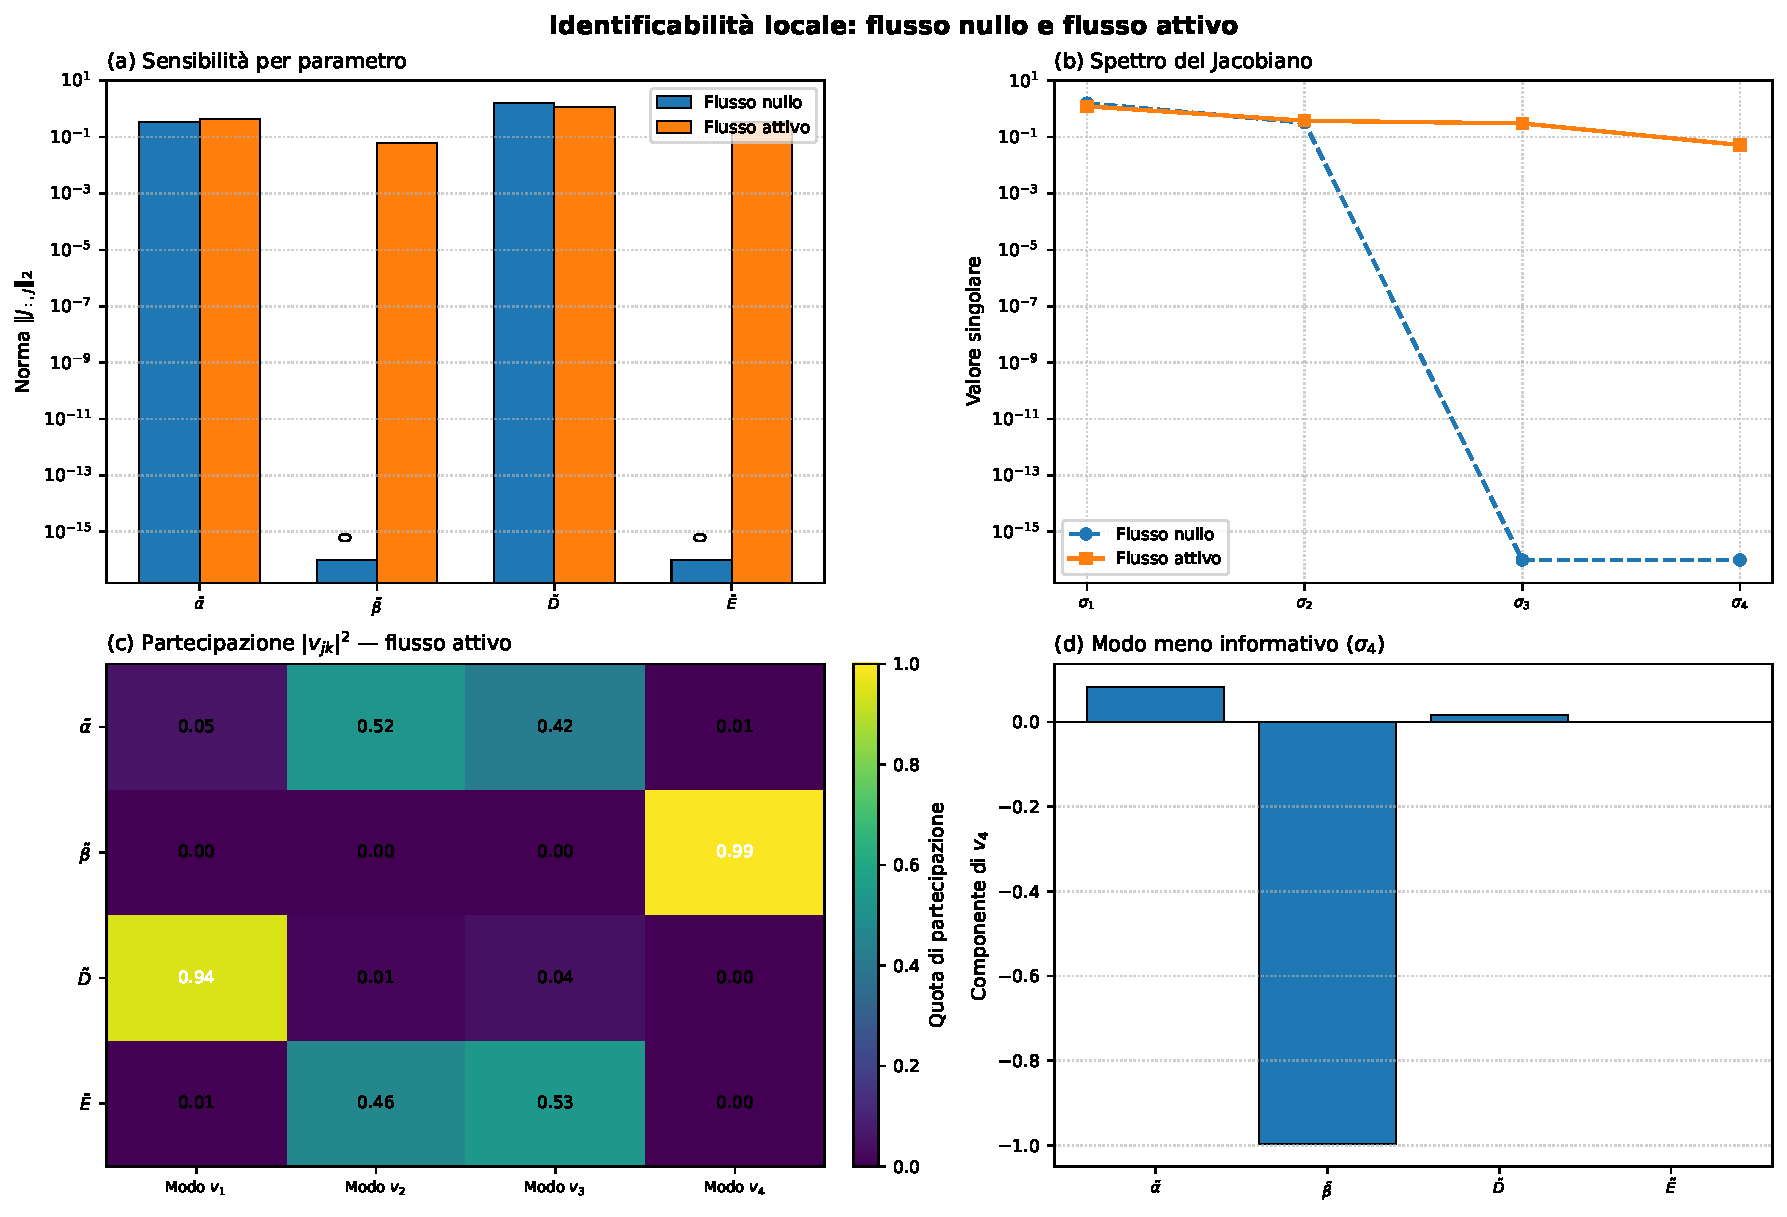
\includegraphics[width=0.85\textwidth]{appendices/figs_C01_local_svd_flow_comparison.pdf}
\caption{Confronto del Jacobiano osservativo a flusso nullo e attivo sul quadrato unitario. Il flusso nullo produce due colonne nulle ($\widetilde\beta$ e $\widetilde E$) e due valori singolari nulli; nel caso attivo, il modo singolare meno informativo resta dominato da $\widetilde\beta$. I pesi sono identità sulle osservazioni adimensionali.}
\label{fig:app-flow-svd-comparison}
\end{figure*}

\begin{figure}[H]
\centering
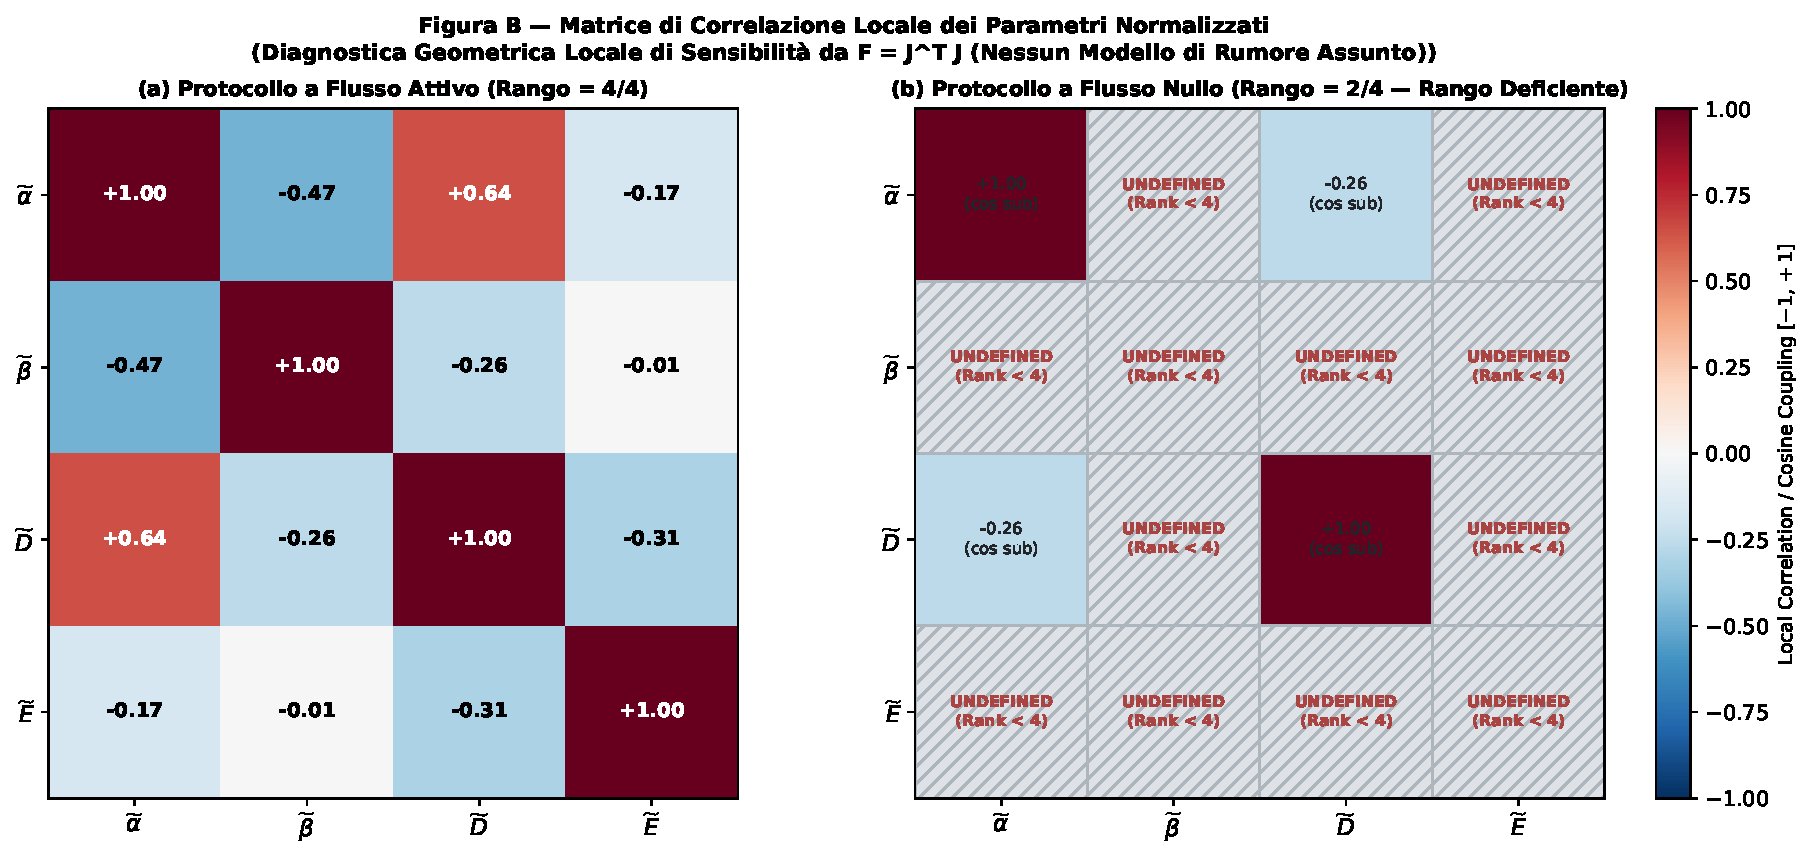
\includegraphics[width=0.85\linewidth]{appendices/figs_C01_local_correlation.pdf}
\caption{Il pannello (a) mostra la matrice di correlazione geometrica locale nel protocollo a flusso attivo; il pannello (b) mostra le similarità coseno tra le sole colonne non nulle nel protocollo a flusso nullo. Le celle tratteggiate indicano quantità non definite perché associate a colonne nulle del Jacobiano. La figura descrive la geometria locale della linearizzazione con pesi identità e non rappresenta correlazioni statistiche posteriori né ellissi di confidenza.}
\label{fig:app-local-geometry}
\end{figure}

\subsection{Transizione di sensibilità rispetto all'eccitazione}
\label{app:flow-transition}

La Tabella~\ref{tab:app-flow-sweep} riporta l'intera scansione del fattore $\kappa_q$. La soglia relativa del rango è $10^{-8}$; il numero di Péclet globale è definito dalla (\ref{eq:peclet-global}).

\begin{table}[H]
\centering
\caption{Scansione completa del Jacobiano sul quadrato unitario al variare del fattore comune di forzamento $\kappa_q$. Le ultime due colonne sono rispettivamente il valore singolare minimo e il numero di condizionamento completo.}
\label{tab:app-flow-sweep}
\small
\begin{tabular}{@{}rrrrrrr@{}}
\toprule
$\kappa_q$ & $\mathrm{Pe}_{\rm glob}$ & Rango & $\sigma_1$ & $\sigma_2$ & $\sigma_3$ & $\sigma_4$\\
\midrule
$0$ & $0$ & $2$ & $1.5833$ & $0.3222$ & $0$ & $0$\\
$10^{-3}$ & $0.003585$ & $4$ & $1.5827$ & $0.3223$ & $3.423\times10^{-4}$ & $5.957\times10^{-5}$\\
$10^{-2}$ & $0.03585$ & $4$ & $1.5775$ & $0.3224$ & $3.422\times10^{-3}$ & $5.954\times10^{-4}$\\
$0.05$ & $0.1793$ & $4$ & $1.5547$ & $0.3232$ & $1.7077\times10^{-2}$ & $2.970\times10^{-3}$\\
$0.10$ & $0.3585$ & $4$ & $1.5271$ & $0.3243$ & $3.4073\times10^{-2}$ & $5.917\times10^{-3}$\\
$0.25$ & $0.8964$ & $4$ & $1.4506$ & $0.3276$ & $8.451\times10^{-2}$ & $1.456\times10^{-2}$\\
$0.50$ & $1.7927$ & $4$ & $1.3457$ & $0.3331$ & $1.661\times10^{-1}$ & $2.801\times10^{-2}$\\
$1$ & $3.5854$ & $4$ & $1.2261$ & $0.3619$ & $2.924\times10^{-1}$ & $4.949\times10^{-2}$\\
$2$ & $7.1708$ & $4$ & $1.2924$ & $0.6129$ & $2.993\times10^{-1}$ & $6.045\times10^{-2}$\\
\bottomrule
\end{tabular}
\end{table}

\begin{table}[H]
\centering
\caption{Numero di condizionamento completo durante la scansione di eccitazione.}
\label{tab:app-flow-conditioning}
\small
\begin{tabular}{@{}rr@{}}
\toprule
$\mathrm{Pe}_{\rm glob}$ & $\kappa(J)$\\
\midrule
$0$ & indefinito ($\operatorname{rank}=2$)\\
$0.003585$ & $26571.23$\\
$0.03585$ & $2649.63$\\
$0.1793$ & $523.54$\\
$0.3585$ & $258.09$\\
$0.8964$ & $99.61$\\
$1.7927$ & $48.03$\\
$3.5854$ & $24.78$\\
$7.1708$ & $21.38$\\
\bottomrule
\end{tabular}
\end{table}

Il rango numerico pieno emerge già quando le colonne meccaniche sono piccole: la scala di $\sigma_4$ e il condizionamento sono quindi più informativi del solo rango.

\subsection{Identificabilità sulla mesh anatomica}
\label{app:anatomical-identifiability}

Sulla mesh BraTS da $3$ mm ($1901$ quadrilateri), con 180 osservazioni della concentrazione e valutazione $Q_1$ diretta, il caso a flusso nullo restituisce rango $2$ e spettro $(0.84817,0.08059,0,0)$. Con forzanti attive lo spettro è $(0.84027,0.05944,0.03197,0.001484)$, il rango è $4$ e $\kappa(J)=566.14$. La componente di $\widetilde\beta$ nel modo singolare meno informativo è $0.9983$. La griglia sensoriale è centrata sul centroide della lesione e ha semi-estensione di $25$ mm in entrambe le direzioni. Il protocollo costituisce una diagnostica locale su un caso anatomico sintetico.

\subsection{Sezioni unidimensionali e scansioni condizionali}

La distinzione interpretativa tra le diverse esplorazioni del paesaggio di costo è essenziale: una sezione unidimensionale (\emph{one-at-a-time}, Figura~\ref{fig:app-oat-slices}) valuta la variazione del funzionale mantenendo rigidi gli altri parametri al valore di riferimento, mentre una scansione condizionale (Figura~\ref{fig:app-beta-conditional}) esplora la dipendenza da $\beta$ fissando gli altri parametri alle stime ottenute da specifiche esecuzioni dell'ottimizzatore. Un profilo ottimizzato consente invece ai parametri di disturbo di compensare la variazione imposta su $\beta$. Per il protocollo considerato, il Jacobiano e i profili sono letti congiuntamente: la stabilità numerica delle derivate non elimina la debole informazione associata alla direzione meno sensibile.

\begin{figure}[htbp]
\centering
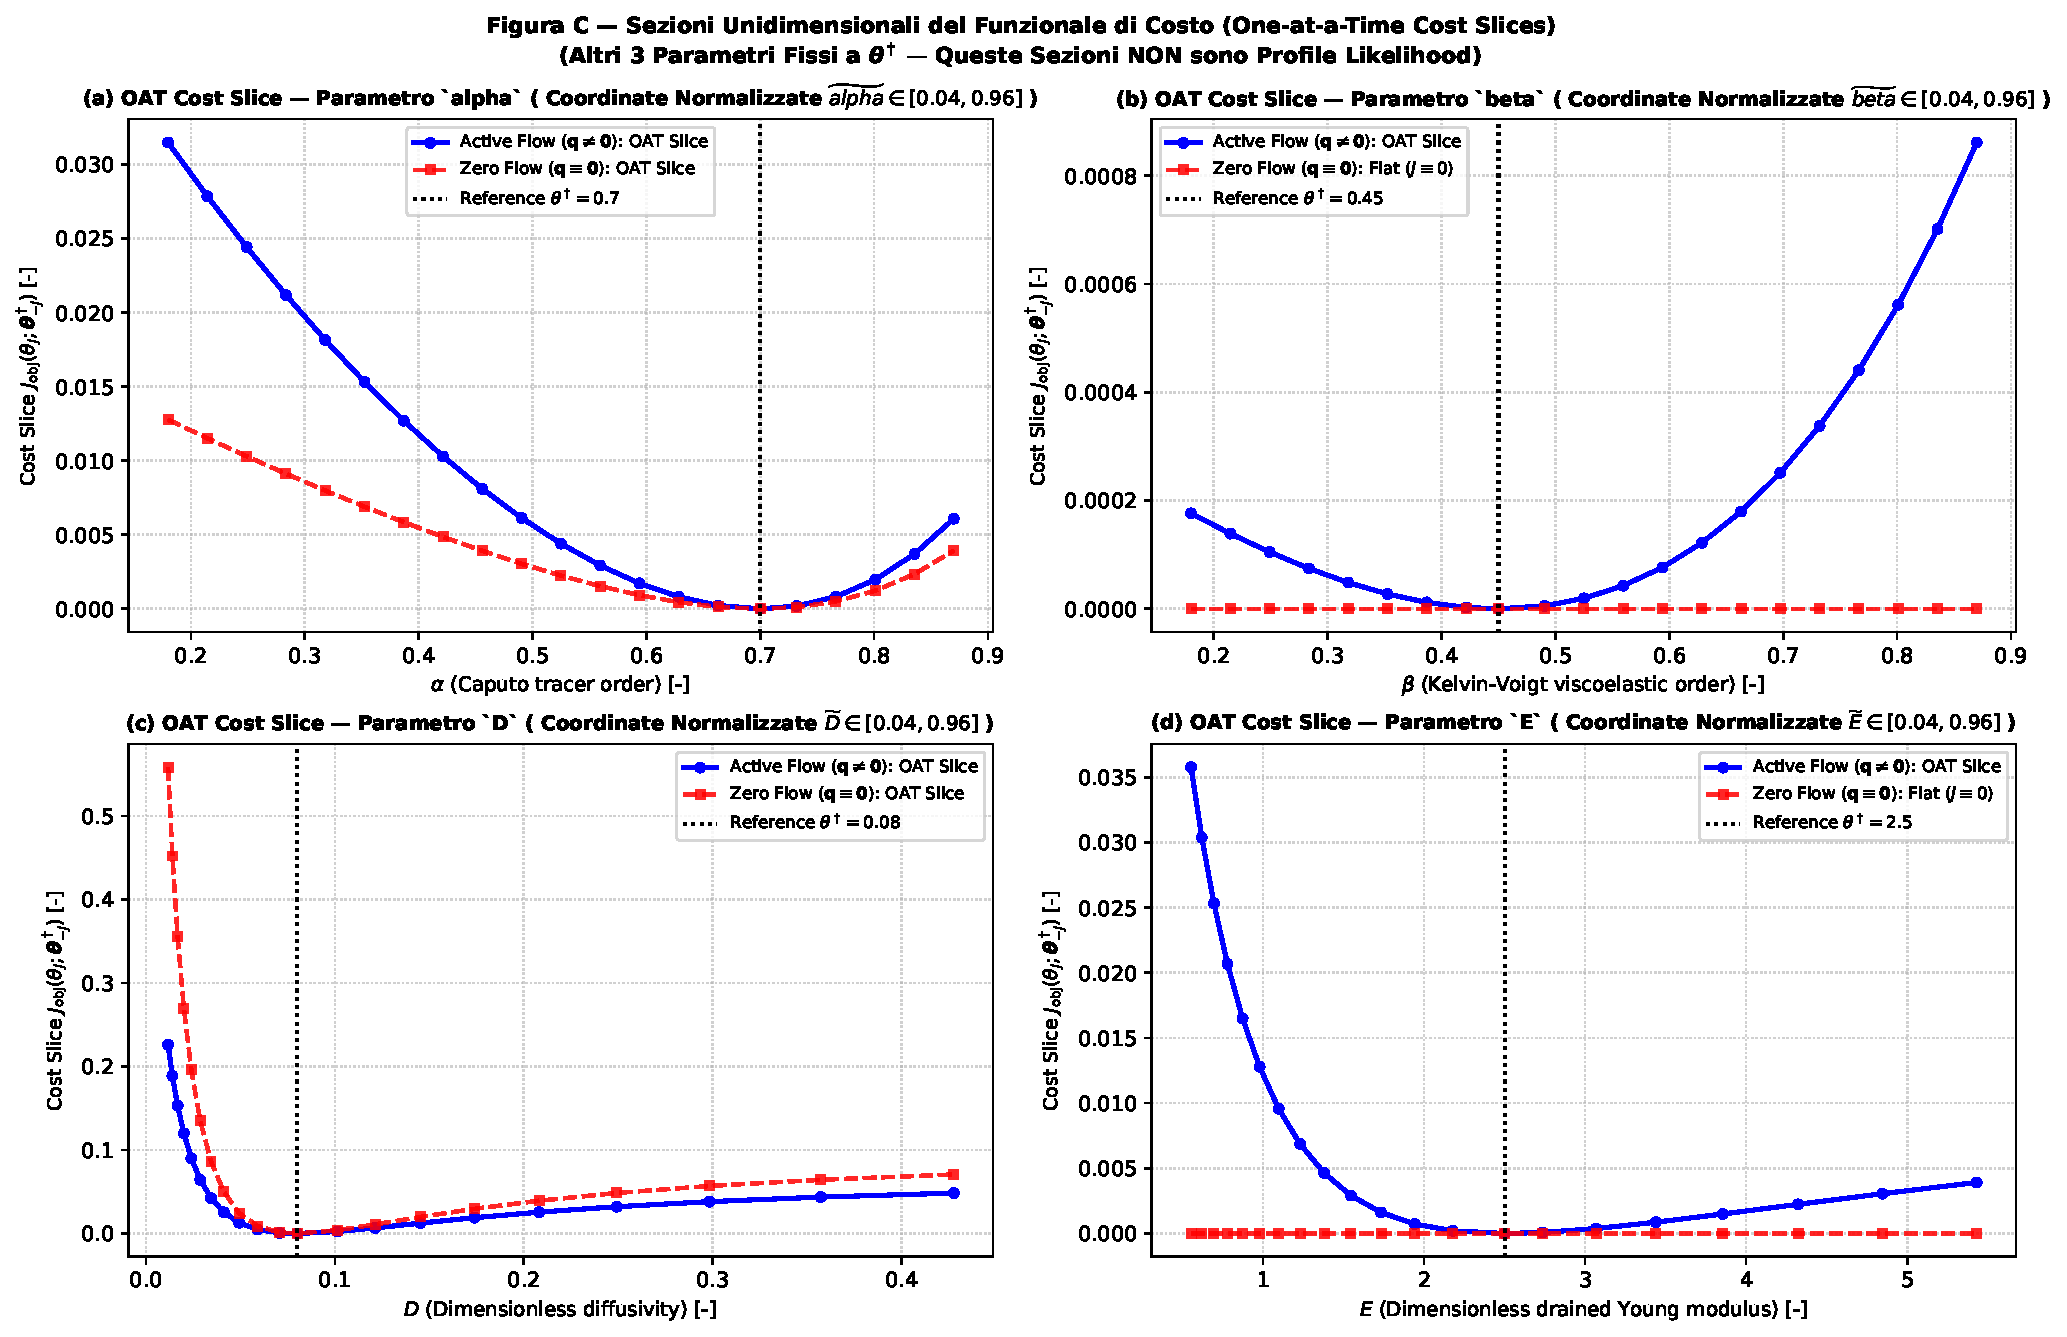
\includegraphics[width=0.8\textwidth]{appendices/figs_C02_one_at_a_time_cost_slices.pdf}
\caption{Sezioni unidimensionali (\emph{one-at-a-time}) del funzionale obiettivo: ciascun parametro varia singolarmente mentre i restanti sono mantenuti fissi al riferimento nominale. I profili piatti a flusso nullo per $\beta$ ed $E$ riflettono la degenerazione strutturale del modello; gli altri parametri sono mantenuti fissi.}
\label{fig:app-oat-slices}
\end{figure}

\begin{figure}[H]
\centering
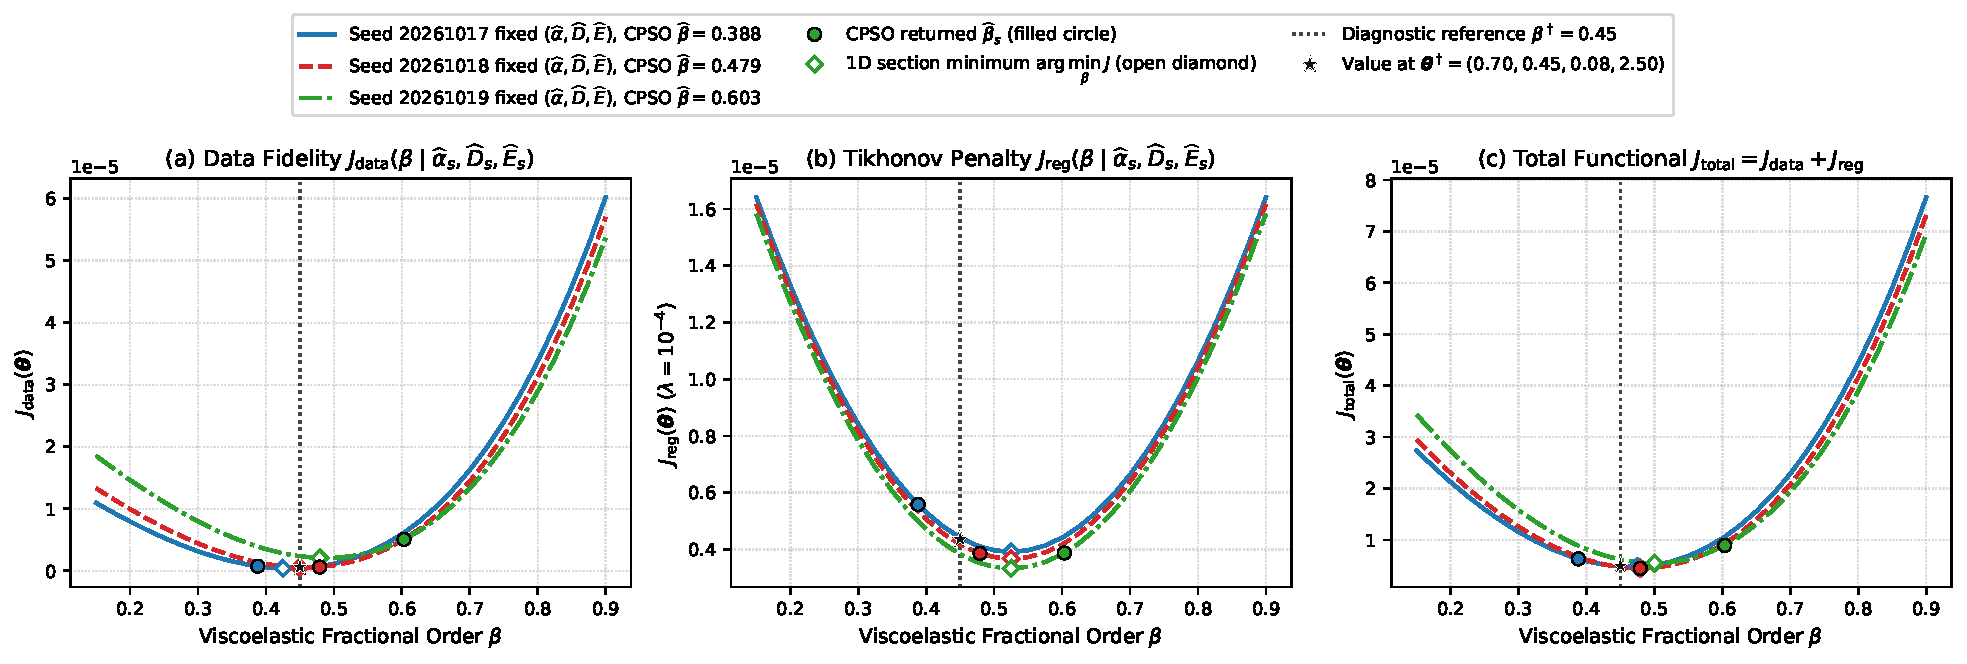
\includegraphics[width=0.8\linewidth]{appendices/figs_C03_beta_conditional_landscape.pdf}
\caption{Sezioni condizionali rispetto a $\beta$ ottenute fissando i parametri complementari ai valori finali delle tre esecuzioni CPSO senza rumore. La figura evidenzia la sensibilità del minimo apparente unidimensionale rispetto al contesto parametrico fissato e non sostituisce il profilo ottimizzato bidirezionale mostrato nella Figura~\ref{fig:beta-profiles}, nel quale i parametri di disturbo vengono ricalibrati ad ogni nodo.}
\label{fig:app-beta-conditional}
\end{figure}